\documentclass{beamer}
\usetheme{Frankfurt}

\usepackage{aliascnt}
\usepackage[spanish]{babel}
\usepackage{amsmath,amsthm,amssymb}
\usepackage{hyperref}
\usepackage{xcolor}
\usepackage{graphicx}
\graphicspath{{assets/}}

% Math environment
\setbeamertemplate{theorem}[ams style]
\deftranslation[to=spanish]{Theorem}{Teorema}
\deftranslation[to=spanish]{Corollary}{Corolario}
\deftranslation[to=spanish]{Lemma}{Lema}
\deftranslation[to=spanish]{Proof}{Demostración}
\deftranslation[to=spanish]{Definition}{Definición}
\deftranslation[to=spanish]{Example}{Ejemplo}
\theoremstyle{remark}
\newtheorem{remark}{Nota}

% Pseudocode environment
\usepackage[ruled,vlined]{algorithm2e}
\renewcommand{\algorithmcfname}{Algoritmo}
\renewcommand{\algorithmautorefname}{Algoritmo}
\renewcommand{\listalgorithmcfname}{Índice de algoritmos}

\title{Curvas Elípticas}
\author{Emanuel Nicolás Herrador}
\institute{Facultad de Matemática, Astronomía, Física y Computación\\Universidad Nacional de Córdoba}
\titlegraphic{
\includegraphics[width=5cm]{logo.png}}
\date{21 de Octubre 2025}

\newcommand{\appendixtitle}{
  \title{Apéndice}
  \subtitle{Material complementario}
}

\begin{document}
\frame{\titlepage}

\AtBeginSection[]{
  \begin{frame}
    \frametitle{Índice}
    \tableofcontents[currentsection]
  \end{frame}
}

\section{Curvas elípticas en un cuerpo finito}
\subsection{Definición y modelos}
\begin{frame}{Definición y modelos}
  \alt<3->{
    Hay muchos modelos para representar ECs con funciones más sencillas.
    Algunos de ellos son:
    \begin{itemize}
      \item<4-> Weierstrass: $y^2 = x^3 + ax + b$ $\rightarrow$ Modelo más general
      \item<5-> Montgomery: $by^2 = x^3 + ax^2 + x$ $\rightarrow$ Puntos de orden $2$
      \item<6-> Twisted Edwards: $ax^2 + y^2 = 1 + dx^2y^2$ $\rightarrow$ Puntos de orden $4$
      \item<7-> Twisted Hessian
      \item<7-> Jacobi intersections 
    \end{itemize}
    \only<8->{
      \begin{remark}
        Montgomery $\leftrightarrow$ Weierstrass con cambio de variable $u := bx - \frac{a}{3}$
        y $v := by$.
      \end{remark}
    }
  }{
    \only<1->{
      \begin{definition}[Forma general]
        Una curva elíptica (EC) es definida en un cuerpo $\mathbb{K}$ con la ecuación:
        \begin{equation*}
          E/\mathbb{K}:\ y^2 + a_1xy + a_3y = x^3 + a_2x^2 + a_4x + a_6 
        \end{equation*}
        donde $a_i \in \mathbb{K}$ ($i=1,2,3,4,6$) y tal que $\Delta \neq 0$ (discriminante).
      \end{definition}
    }
    \only<2->{
      Hay muchos modelos para representar ECs con funciones más sencillas.
    }
  }
\end{frame}

\begin{frame}{Puntos en EC}
  \only<1->{
    \begin{definition}[Punto en la curva]
      Sea $E/\mathbb{F}_p$ EC y $e \geq 1$, decimos que $(x_1,y_1)$ con $x_1,y_1\in\mathbb{F}_{p^e}$
      es un punto en la curva $E$ si $(x_1,y_1)$ satisface la ecuación de $E$.
    \end{definition}
  }
  \begin{itemize}
    \item<2-> Se incluye un punto especial $\mathcal{O}$ llamado \textit{punto al infinito}.
    \item<3-> $E(\mathbb{F}_{p^e})$ denota el conjunto de puntos de $E$ sobre $\mathbb{F}_{p^e}$
      incluyendo $\mathcal{O}$.
    \item<4-> El número de puntos de una EC es cercano a $p^e + 1$:
      \begin{theorem}[Hasse]
        $\left|E(\mathbb{F}_{p^e})\right| = p^e + 1 - t$ para algún entero $t$ tal que
        $|t| \leq 2\sqrt{p^e}$.
      \end{theorem}
  \end{itemize}
\end{frame}

\subsection{Operaciones}
\begin{frame}{Operaciones: Suma}
  Supongamos $P,Q,R \in E(\mathbb{F}_{p^e})$.
  \begin{itemize}
    \item<1-> Denotamos la suma como $\boxplus$
    \item<2-> La identidad es $\mathcal{O} \rightarrow \forall P, P \boxplus \mathcal{O} = \mathcal{O} \boxplus P = P$.
    \alt<5->{
    }{
      \item<3-> Supongamos $P \neq Q$ y queremos $P + Q = R$.
        Gráficamente la idea es:
        \begin{enumerate}
          \item<3-> Dibujar la línea que cruza $P$ y $Q$.
          \item<3-> Denotar $-R$ al tercer punto intersecado en la curva por la línea.
          \item<3-> Trazar la recta vertical en $-R$, de tal modo que el punto intersecado 
            en la curva es $R$.
        \end{enumerate}
      \item<4-> Si $P = Q$, el \textit{doblado de puntos} es el mismo proceso pero trazando 
        la tangente a $P$.
    }
  \end{itemize}
  \alt<6->{
    \begin{remark}
      Es un grupo abeliano porque cada punto tiene un inverso aditivo, la suma es 
      asociativa y también conmutativa.
    \end{remark}
  }{
    \only<5->{
      \begin{center}
        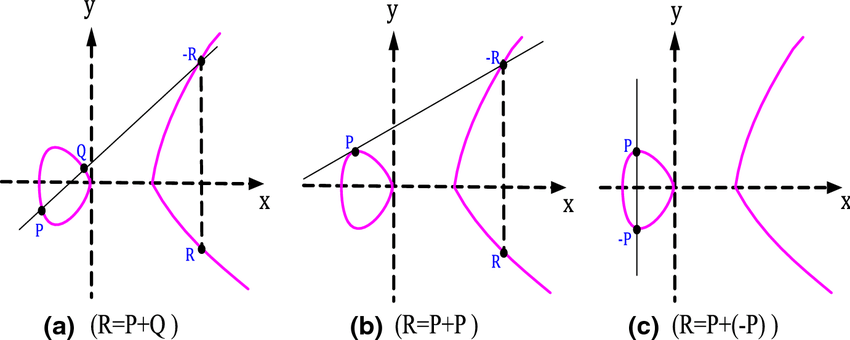
\includegraphics[width=0.9\textwidth]{point-addition.png}
      \end{center}
    }
  }
\end{frame}

\begin{frame}{Operaciones: Multiplicación por escalar}
  Supongamos $P \in E(\mathbb{F}_{p^e})$
  \begin{itemize}
    \item<1-> Denotamos $kP := \overbrace{P \boxplus \dots \boxplus P}^{k\text{ veces}}$
    \item<2-> Se puede computar en $O(2\log_2 k)$ operaciones de grupo usando los algoritmos 
      de Montgomery o de Joye.
  \end{itemize}
  \only<3->{
      \begin{algorithm}[H]
        \DontPrintSemicolon
        \footnotesize
        \caption{Idea similar a \textit{binexp}}
        \KwIn{$P \in E(\mathbb{F}_{p^e}),\ k \in \mathbb{Z^+}$}
        \KwOut{$kP \in E(\mathbb{F}_{p^e})$}
        $kP = \mathcal{O},\ b = P$ \\
      \While{$k > 0$}{
        \If{$k \& 1$}{
          $kP \leftarrow kP \boxplus b$
        }
        $b \leftarrow 2b$ \\
        $k \leftarrow (k \gg 1)$
      }
      \KwRet{$kP$}
    \end{algorithm}
  }
\end{frame}

\section{Curvas elípticas en criptografía (ECC)}
\subsection{Definiciones}
\begin{frame}{EC en criptografía}
  Sea $E/\mathbb{F}_p$ una EC, consideraremos:
  \begin{itemize}
    \item<1-> $E(\mathbb{F}_p)$ cícliclo, i.e., generado por algún punto $P \in E(\mathbb{F}_p)$.
    \item<2-> Asunción de que los siguientes problemas son \textit{difíciles} en 
      el grupo:
      \begin{itemize}
        \item Logaritmo discreto (DL)
        \item Computational Diffie-Hellman (CDH)
        \item Decision Diffie-Hellman (DDH)
      \end{itemize}
    \item<3-> Además de otros usos en esquemas de pairings o isogenies, pueden 
      aplicarse en los criptosistemas vistos anteriormente con grupos finitos.
  \end{itemize}
\end{frame}

\subsection{DL y curvas inseguras}
\begin{frame}{Análisis de DL y curvas inseguras}
  \alt<2->{
    \begin{itemize}
      \item<2-> El algoritmo para romper DL en un grupo cíclico de orden $q$ usa al menos 
        $O(\sqrt{q})$ operaciones de grupo.
        En el caso de ECC, tenemos $q := \left|E(\mathbb{F}_p)\right|$.
      \item<3-> No todas las curvas son seguras:
        \begin{itemize}
          \item Si $|E(\mathbb{F}_p)| = q_1 \cdot \dots \cdot q_n$ con $q_i$ primos tal que $q_i \leq q_{\max}$,
            entonces existe un algoritmo que resuelve DL en $\tilde{O}(\sqrt{q_{\max}})$.
          \item Si $|E(\mathbb{F}_p)| = p$ entonces DL es resoluble en tiempo polinomial.
        \end{itemize}
      \item<4-> En particular para $E/\mathbb{F}_{p^e}$, existe un algoritmo que lo resuelve
        en un tiempo conjeturado de $\tilde{O}\left(p^{2-\frac{2}{e}}\right)$.
        Por ello, se suele tomar $p$ suficientemente grande para hacerlo impráctico
        ($p \geq 2^{256}$ es suficiente).
    \end{itemize}
  }{
    \only<1->{
      \begin{definition}[Problema DL]
        Sea $P \in E(\mathbb{F}_p)$ de orden $q$ (i.e., tal que $qP = \mathcal{O}$).
        Son dados $(P,q,Q)$ donde $Q := \alpha P$ para algún $\alpha\in\mathbb{Z}_q$ y 
        se pretende computar $\alpha$, el logaritmo discreto de $Q$ base $P$
        en $E(\mathbb{F}_q)$.
      \end{definition}
    }
  }
\end{frame}

\subsection{Curvas específicas a usar}
\begin{frame}{secp256r1}
  \begin{itemize}
    \item Conocida como Curva P256 en el estándar de NIST 
    \item Primo $p_r := 2^{256} - 2^{224} + 2^{192} + 2^{96} - 1$
    \item Forma de Weierstrass $y^2 = x^3 - 3x + b$ con $b$ de $255$-bits dado por
      \begin{equation*}
        \begin{aligned}
          b := &\texttt{5ac635d8 aa3a93e7 b3ebbd55 769886bc}\\
               &\texttt{651d06b0 cc53b0f6 3bce3c3e 27d2604b}
        \end{aligned}
      \end{equation*}
      elegido de un algoritmo determinístico público con una constante $S$ (seed)
      dada.
    \item $|E(\mathbb{F}_{p_r})|$ es primo cercano a $p_r$
    \item Se especifica un punto $G_r$ que genera el grupo $E(\mathbb{F}_{p_r})$
  \end{itemize}
  \only<2->{
    \begin{remark}
      Si una organización elige/setea el $S$, estamos confiando de que no lo haga 
      de modo tal que sea fácil para ellos romper DL el los grupos generados.
    \end{remark}
  }
\end{frame}
\begin{frame}{secp256k1}
  \alt<2>{
    \begin{itemize}
      \item Es una curva de Koblitz, por lo que $\exists \omega \neq 1 \in \mathbb{F}_p : \omega^3 = 1$.
      \item Sea el mapeo $\phi:\mathbb{F}_p^2\to\mathbb{F}_p^2$ dado por $\phi(x,y):=(\omega x,y)$, entonces:
        \begin{itemize}
          \item Es un mapeo de $E(\mathbb{F}_p)$ en $E(\mathbb{F}_p)$, i.e., homomorfismo de grupo.
          \item Luego, $\exists \lambda \in \mathbb{Z}_q : \forall P \in E(\mathbb{F}_p), \phi(P) = \lambda \cdot P$.
            Este es la raíz no trival en $1 + \lambda + \lambda^2 = 0$.
        \end{itemize}
      \item Dado $\alpha \in \mathbb{Z}_q$, podemos encontrar $|\tau_i| \leq 2q^{\frac{1}{3}}$ tal que
        \begin{equation*}
          \alpha = \tau_0 + \tau_1\lambda + \tau_2\lambda^2
        \end{equation*}
      \item Luego, $\alpha P$ se computa como $\tau_0 \cdot P + \tau_1 \cdot \phi(P) + \tau_2 \cdot \phi^2(P)$,
        reduciendo su complejidad.
    \end{itemize}
  }{
    \begin{itemize}
      \item Primo $p_k := 2^{256} - 2^{32} - 2^{9} - 2^{8} - 2^{7} - 2^{6} - 2^{4} - 1$
      \item Forma de Weierstrass $y^2 = x^3 + 7$
      \item $|E(\mathbb{F}_{p_k})|$ primo cercano a $p_k$
      \item Se especifica un punto $G_k$ que genera a $E(\mathbb{F}_{p_k})$
    \end{itemize}
  }
\end{frame}
\begin{frame}{Curve25519}
  \alt<4->{
    \begin{itemize}
      \item Diseñada para soportar operaciones de grupo optimizadas y ser twist secure 
      \item Primo $p := 2^{255} - 19$
      \item Forma de Montgomery: $y^2 = x^3 + 486662 \cdot x^2 + x$
      \item El cofactor de la curva es $8$ (i.e., $|E(\mathbb{F}_p)| = 8k$ con $k$ primo)
      \item Generada por $P = (x_1,y_1)$ con $x_1 = 9$
    \end{itemize}
  }{
    \only<1->{
      \begin{definition}[Twist]
        Sean $E/\mathbb{F}_p$ una EC y $c \in \mathbb{F}_p$ no residuo cuadrático.
        Entonces si la curva $E$ es $y^2 = x^3 + ax + b$, luego su twist/torcedura
        $\tilde{E}$ es $cy^2 = x^3 + ax + b$.
      \end{definition}
    }
    \only<2->{
      \begin{definition}[Security twist]
        Una curva $E/\mathbb{F}_p$ es \textit{twist secure} si DL es difícil en 
        $E(\mathbb{F}_q)$ y en $\tilde{E}(\mathbb{F}_q)$.
      \end{definition}
    }
    \only<3->{
      \textbf{Ejemplo de importancia}:
      Supongamos oblivious PRF donde Bob tiene SK $\alpha\in\mathbb{Z}_q$ y dado $P \in E(\mathbb{F}_p)$
      retorna $\alpha P$. Por optimización, a veces solo se pide $P_x$ por lo que no
      se corrobora pertenencia.
      Luego, podemos considerar $P \in \tilde{E}(\mathbb{F}_q)$ y como DL es fácil 
      en el twist, obtenemos $\alpha$.

      \begin{center}
        \textcolor{red}{\textbf{Demo}: Twist and shout (RCSC 2023 - Noruega)}
      \end{center}
    }
  }
\end{frame}

\subsection{Ejemplos de uso}
\begin{frame}{Ejemplos de uso}
  Algunos esquemas de ejemplo donde se usan las EC son:
  \begin{itemize}
    \item ECDH: variante de Diffie-Hellman
    \item ECDSA: variante de DSA (firma)
  \end{itemize}

  La ventaja de EC por sobre esquemas basados en RSA o factorización es que obtiene
  la misma seguridad con claves más cortas.
\end{frame}

\end{document}
